\documentclass{article}
\usepackage[utf8]{inputenc}
\usepackage{graphicx}
\usepackage{hyperref}
\begin{document}

\title{How To Sigi}
\author{Ekter}
\date{August 2024}
\maketitle


\section{Introduction}

The Sigi is a robot from Pololu(the Balboa 32U4 board) combined with a Raspberry Pi.
It is a segway-based robot(inverted pendulum on wheels), so it has two parallel wheels.
It is an unstable system, so it is interesting to try the stability of different controllers.

This document is a guide to how to use the Sigi robot.
It attempts to be a comprehensive guide to the robot, from the hardware to the software,
including various useful resources for understanding the operation of all different parts of the system.
It will also include some info on problems caused by the current design of the system and,
when possible, details on how to fix them.

If detailed documentation is needed, the \href{file://Sigi_documentation_part1.pdf}{Sigi2.0: Documentation}
is quite complete on anything related to hardware.


\section{Hardware}

\subsection{Different parts overview}
\subsubsection{Balboa 32U4}
The Balboa 32U4 is the main board of the robot.
It can be programmed like an Arduino board using the Arduino IDE for example, by plugging the board to a
computer using its micro-USB interface.
It has a lot of components, but the most important are:
\begin{list}{-}{}
    \item The two motor drivers, which are used to control the two motors of the robot.

    \item The IMU, which is used to measure the angle of the robot.

    \item The encoders, which are used to measure the speed of the motors.
\end{list}

Other notable components are:

\begin{list}{-}{}
    \item The buzzer, which can be used to make sounds.

    \item The buttons, which can be used to interact with the robot.

    \item The LEDs, which can be used to show information to the user.

    \item The battery monitor, which can be used to measure the battery level.

    \item The communication interfaces and GPIOs, which can be used to connect the board to
        other devices.

    \item A reset button on the side of the board.
\end{list}

\subsubsection{Raspberry Pi3B+}
The Raspberry Pi are a series of small single-board computers.
The Raspberry Pi 3B+ is the one used in the Sigi robot.
It is used to run the high-level software of the robot.

The Pi 3B+ in particular features a wi-fi interface which can be used to connect to the robot
remotely.

\subsection{Sigi power management}
The Sigi is intended to be used with cells, but can also be powered by its micro-USB interface,
with an USB power bank for example.
But the micro-USB interface is not fed into the motors, so a jumper wire has been installed on the
Sigi bypass the battery regulator and feed the motors with the micro-USB power when connected.
This jumper is located between the VSW and the 5V pins near the micro USB port of the Balboa board.

\begin{center}
    % \begin{figure}                % I don't know how to use this
        
        
        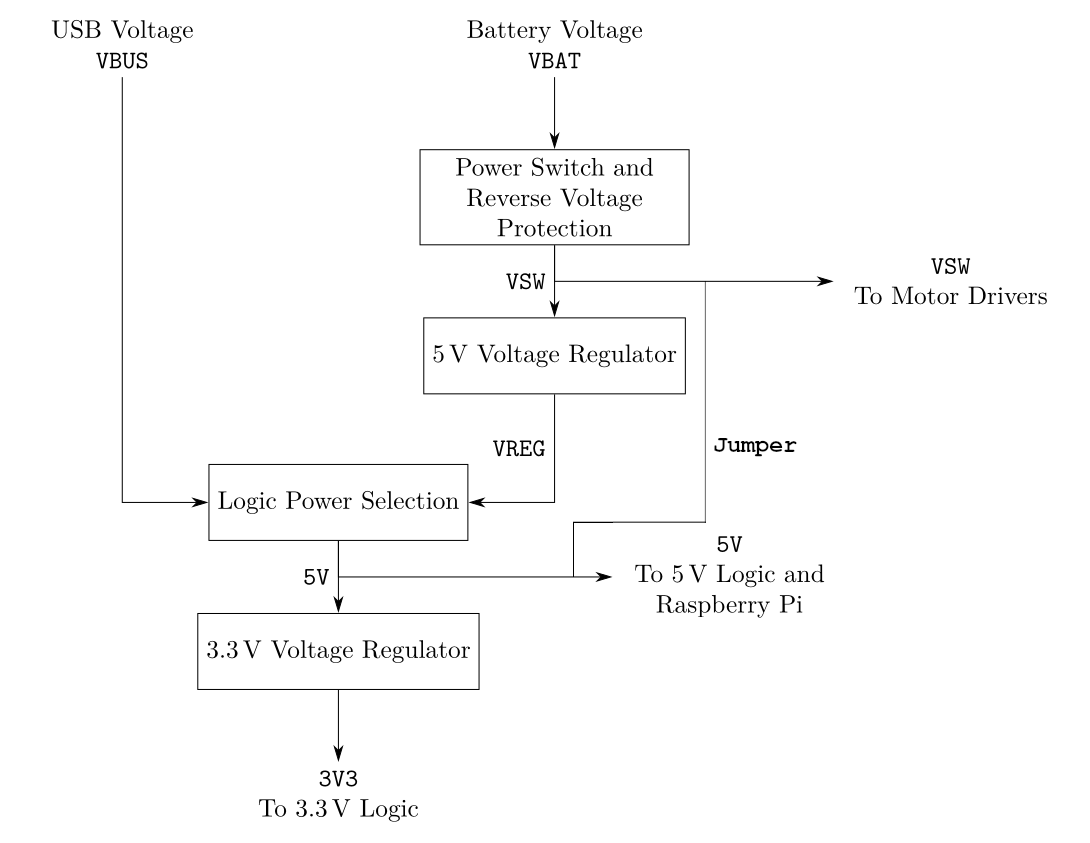
\includegraphics{img/power.png}

        Figure 1: The jumper wire on the Sigi robot voltage lines.
    % \end{figure}

\end{center}

This is fine most of the time, but it can occasionally cause problems.
If the current drawn by the system is too high(high speed change in the motors+heavy 
computations on the Raspberry Pi), the voltage of the 5V logic will drop, causing
resets of the Balboa board. Fortunately this reset stops the motors, so the voltage will rise
again, so the Raspberry Pi, requiring less voltage, won't reboot. But since the Balboa board
resets, the encoders will reset, which may cause the robot to lose its position if it was not
saved by the Raspberry Pi.

One solution could be using a battery, but the jumper prevents the battery's voltage from being
too high, since it is connected to the 5V logic and the Raspberry Pi. Experimentally, the max
voltage was measured around 7.5V, but it was already causing consumption and heating problems on
the regulator. In normal conditions, the voltage should be capped at 7V for safer operation.
This also implies a minimal voltage. In fact, the voltage protection removes approximately 10\%
of the voltage, so in order to achieve the 5V logic, the voltage should be at least 5.5V.
Some problems have been observed at 5.5V, but their exact cause is unknown. It could be the
voltage regulator not having enough power when the motors are running for example.
So the optimal voltage of a battery should be between 6 and 7V. A higher voltage battery
with a voltage regulator would also be ok.

*note: insert power diagram

Removing the jumper would help if using a battery, but of course it would prevent to go back to
using an USB power bank without soldering the jumper back.

Side note:
It is what I have done with my Sigi(14), and I alternate between the battery and the USB power
for tests and operation.

Another solution could be to use another Raspberry Pi with less current consumption. For example,
a Pi Zero W has almost the same wireless capabilities, but consumes less power. However,
the computational power is also reduced, so it may not be enough for some applications.

\section{Software}
The current design of the Sigi is like this:

\begin{center}

    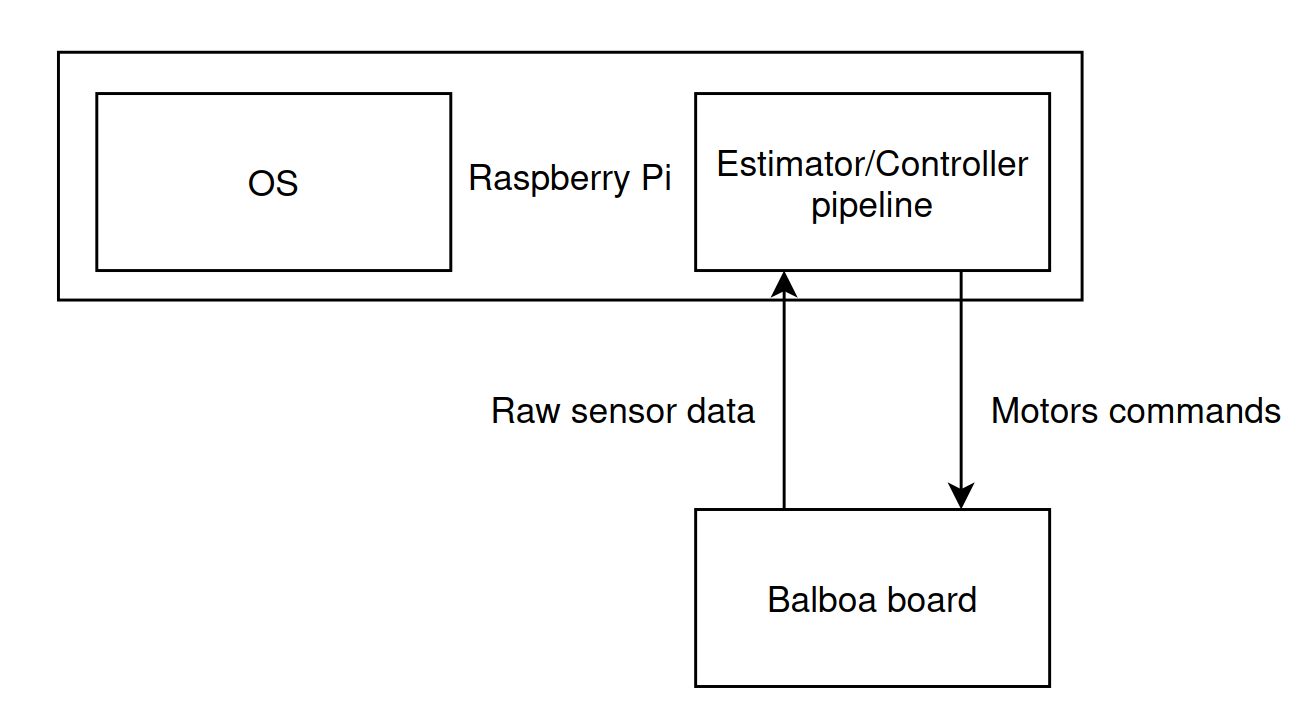
\includegraphics[scale=0.2]{img/software.png}

    Figure 2: Software overview

\end{center}

The Balboa 32U4 is only used to get the raw sensor data, and the controller is running on the
Raspberry Pi. The Balboa board could also be used to run the controller, but using the Raspberry
Pi allows for more complex computations and easier debugging. The possibility of using the Python
language is also a plus, see 3.3 for more details.

\subsection{Interface between the Raspberry Pi and the Balboa board}

Communication between the Raspberry Pi and the Balboa board is needed for multiple purposes
that cannot be done directly with the Raspberry Pi :

\begin{list}{-}{}
    \item Reading the state of the robot from the sensors
    \item Sending commands to the motors, LEDs or other actuators
\end{list}

The communication is done via the I2C interface.
Other communication media could possibly be used, but have not been documented by Pololu,
using an USB or UART interface for example.
The current protocol used is actually a variant of the I2C protocol, the
\href{https://en.wikipedia.org/wiki/System_Management_Bus}{SMBUS} protocol.
The Raspberry Pi is the master and the Balboa board is a slave.
The IMU is also a slave, since it is accessed directly by the Raspberry Pi without
going through the Balboa board's micro controller.

\begin{center}

    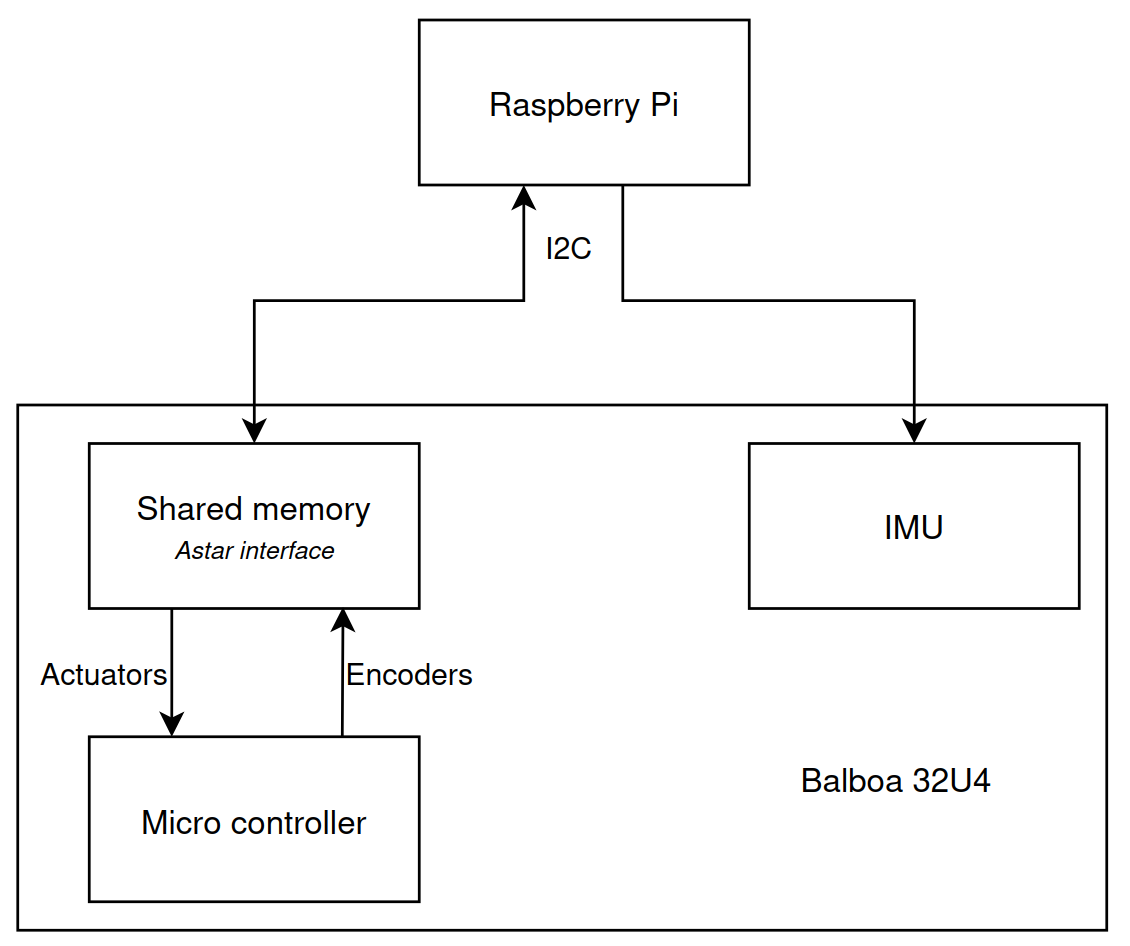
\includegraphics[scale=0.25]{img/i2c-interface-diagram.png}

    Figure 2: I2C diagram of the Balboa/Pi interface
    % TODO make this correctly(shared memory etc)

\end{center}
*note TODO make this correctly(shared memory etc)

\subsubsection{Balboa board}

The Balboa board's micro-controller has to read the shared memory(note: it is called a buffer in
the code but it is technically not one) to know the orders from the Raspberry Pi, and update its
right fields so that the encoders ticks can be read from the Raspberry Pi.
The default example code from Pololu handles these tasks quite well. A notable possible
improvement could be improving it to read the last saved value on the buffer after resets to
recover more efficiently.

\end{document}
